% Generador, buffer y consumidor: por qué agregar buffering baja el tiempo
% muerto. Arriba, un buffer de un lugar con handshake (el esquema de
% arm/congelar/re-armar, análogo a un MCP): lleno, la entrada queda congelada
% hasta el re-armado. Abajo, un buffer de K lugares con dos punteros (el ring,
% análogo a una FIFO asincrónica). El MISMO tren de nueve eventos en las dos, con
% servicio fijo τ: en (a) se pierden cinco, en (b) con K = 3 ninguno.
% Es un esquema, no una medición: los números están en
% docs/buffering_y_tiempo_muerto.md.
%
% Compilar:   pdflatex buffering_generador_consumidor.tex
%             pdftocairo -svg buffering_generador_consumidor.pdf buffering_generador_consumidor.svg
%
\documentclass[border=0pt,tikz]{standalone}
\usepackage[utf8]{inputenc}
\usepackage[T1]{fontenc}
\usepackage{lmodern}
\usepackage[none]{hyphenat}
% Estilo común de las figuras TikZ (panoramas y diagramas de bloques).
%
% Cada figura lo incluye con \input{../../figuras/estilo_tikz.tex} (las figuras
% viven en docs/<módulo>/figuras/). Un solo lugar para la paleta, los estilos de
% bloque y el formato de los parámetros: si cambia algo acá, cambia en todas.
%
% La paleta es la misma de docs/figuras/estilo_svg.py y de PALETA en
% modulos/mk/datasheet.py; si se toca un color, se toca en los tres.
%
% Requiere: \usepackage{tikz} (lo da la clase standalone con la opción tikz).

\usetikzlibrary{arrows.meta,positioning,calc,fit,backgrounds,shapes.multipart,
                decorations.markings,shadows}

% ---------------------------------------------------------------- colores ---
\definecolor{azul}{RGB}{108,172,228}      % acondicionamiento
\definecolor{verde}{RGB}{110,214,142}     % captura / histogramas en BRAM
\definecolor{amarillo}{RGB}{252,232,160}  % trigger
\definecolor{naranja}{RGB}{252,206,160}   % camino a DDR
\definecolor{grisr}{RGB}{226,226,226}     % compartido / infraestructura
\definecolor{rojo}{RGB}{240,128,128}      % bus del sistema

% ---------------------------------------------------------------- estilos ---
\tikzset{
  >={Stealth[length=2.4mm,width=1.8mm]},
  % fondo blanco siempre: el SVG se ve igual en modo claro y oscuro
  fondo/.style   = {show background rectangle, inner frame sep=8pt,
                    background rectangle/.style={fill=white, draw=none}},
  bloque/.style  = {draw=black, line width=0.6pt, rounded corners=2pt,
                    align=center, text width=2.2cm, minimum height=1.15cm,
                    inner sep=2pt, font=\scriptsize, fill=#1},
  datos/.style   = {bloque=azul!35},
  trig/.style    = {bloque=amarillo},
  captura/.style = {bloque=verde!55},
  ddr/.style     = {bloque=naranja!70},
  comp/.style    = {bloque=grisr},
  bus/.style     = {bloque=rojo!45},
  % lógica escrita dentro del módulo, sin submódulo propio
  etapa/.style   = {bloque=#1, line width=0.5pt},
  etapa/.default = verde!20,
  % lo que el bitstream no trae (atado a cero, stub, salida muda)
  mudo/.style    = {bloque=white, draw=black!45, dashed, text=black!55},
  %
  % BLOQUE CON PARÁMETROS, en el formato del datasheet: el encabezado lleva el
  % nombre y los parámetros con que lo instancia el padre (NOMBRE=valor, en
  % monoespaciada, uno por línea); el cuerpo, más claro, lo que hace.
  %   \node[datos, param={azul!35}{azul!12}] {\blk{nombre}{} \prm{A=1\\B=2}
  %                                            \nodepart{two} función};
  param/.style 2 args = {rectangle split, rectangle split parts=2,
                         rectangle split part fill={#1, #2}},
  %
  flujo/.style   = {->, line width=0.8pt},
  ctrl/.style    = {->, line width=0.6pt, black!65},
  % la línea que pasa por encima en un cruce: un halo blanco la separa
  cruce/.style   = {preaction={draw=white, line width=3.4pt, -}},
  % marca de ancho de bus: barra oblicua a mitad de la flecha, con el número
  % encima. \draw[flujo, ancho=14] ...; para otra posición, ancho en=0.3.
  ancho/.style   = {decoration={markings, mark=at position \anchopos with {
                      \draw[line width=0.6pt, -] (-0.1,-0.14) -- (0.1,0.14);
                      \node[font=\scriptsize, above=1.5pt] {#1};}},
                    postaction={decorate}},
  % la misma marca en una flecha vertical: el número va a la derecha
  anchov/.style  = {decoration={markings, mark=at position \anchopos with {
                      \draw[line width=0.6pt, -] (-0.14,-0.1) -- (0.14,0.1);
                      \node[font=\scriptsize, right=3pt] {#1};}},
                    postaction={decorate}},
  ancho en/.code = {\def\anchopos{#1}},
  sen/.style     = {font=\scriptsize\ttfamily, inner sep=1.5pt},
  nodo/.style    = {font=\tiny\ttfamily, inner sep=1pt, black!75},
  pin/.style     = {font=\scriptsize, align=center, inner sep=1pt},
  grupo/.style   = {draw=black!55, dashed, line width=0.7pt, rounded corners=4pt},
  canal/.style   = {grupo},
  contenedor/.style = {draw=black!80, line width=1.0pt, rounded corners=6pt},
  % marca numerada: cada número es una fila de la tabla del documento
  marca/.style   = {circle, fill=black, text=white, font=\scriptsize\bfseries,
                    inner sep=0pt, minimum size=4.3mm},
  %
  % DECISIONES (docs/mca/vista_general_mca.md). Cada opción es un bloque, todas
  % entran a un mux (\muxdec, abajo) y el registro que elige entra por abajo.
  % la opción que trae el reset (el comportamiento histórico): borde doble
  defecto/.style = {double=white, double distance=0.8pt, line width=0.45pt},
  % rótulo de la decisión, el mismo Dn del panorama y del documento
  decision/.style = {circle, fill=black, text=white, font=\small\bfseries,
                     inner sep=0pt, minimum size=7mm},
  %
  % LÓGICA (docs/mca/figuras/contabilidad/ y los detalles de las decisiones)
  % registro: caja gris con el triángulo de reloj en el borde de abajo
  registro/.style = {draw=black, line width=0.6pt, fill=grisr, align=center,
                     font=\scriptsize, inner sep=2pt, minimum width=#1,
                     minimum height=0.85cm,
                     path picture={\draw[line width=0.5pt]
                       ([xshift=-1.1mm]path picture bounding box.south) --
                       ([yshift=1.6mm]path picture bounding box.south) --
                       ([xshift=1.1mm]path picture bounding box.south);}},
  registro/.default = 0.8cm,
  % condición de una cadena if / else-if: "sí" sale a la derecha, "no" abajo
  pregunta/.style = {draw=black, line width=0.5pt, rounded corners=7pt,
                     fill=white, font=\scriptsize\ttfamily, align=center,
                     inner sep=2.5pt, minimum height=0.62cm, text width=#1},
  pregunta/.default = 1.9cm,
  si/.style      = {font=\tiny, inner sep=1pt, above, pos=0.12},
  no/.style      = {font=\tiny, inner sep=1pt, left, pos=0.45},
  %
  titulo/.style  = {anchor=north west, font=\small, inner sep=4pt, align=left},
  rotulo/.style  = {anchor=north west, font=\scriptsize\itshape, black!70,
                    inner sep=2pt, align=left},
}

% submódulo: nombre en monoespaciada; lógica propia: nombre en romana
\newcommand{\blk}[2]{{\ttfamily\bfseries #1}\\[1pt]#2}
\newcommand{\etq}[2]{{\bfseries #1}\\[1pt]#2}
\newcommand{\punto}[1]{\fill (#1) circle (1.3pt);}

% Parámetros en el formato del datasheet: NOMBRE=valor en monoespaciada, una
% entrada por celda, hasta cuatro columnas. Una columna: \prm{A=1\\B=2};
% dos: \prm{A=1 & B=2\\C=3}.
\newcommand{\prm}[1]{{\ttfamily\fontsize{5.6}{6.6}\selectfont
  \begin{tabular}{@{}l@{\hspace{7pt}}l@{\hspace{7pt}}l@{\hspace{7pt}}l@{}}#1\end{tabular}}}

\def\anchopos{0.5}

% Mux de una decisión: trapecio con el lado ancho (las entradas) a la izquierda.
% #1 = nombre, #2 = centro, #3 = alto en cm. Deja tres coordenadas:
%   (#1-in)  centro del lado de entradas: las flechas llegan a (#1-in |- opcion.east)
%   (#1-out) la salida
%   (#1-sel) mitad del lado de abajo: por ahí entra el registro que elige
% El rótulo de adentro es opcional: \muxdec{m}{(4,0)}{3.6} y después
% \node[...] at (m) {...}.
\newcommand{\muxdec}[3]{%
  \path #2 coordinate (#1);
  \draw[line width=0.6pt, fill=grisr]
    ($(#1)+(-0.45,{#3/2})$) -- ($(#1)+(0.45,{#3/2-0.35})$) --
    ($(#1)+(0.45,{-#3/2+0.35})$) -- ($(#1)+(-0.45,{-#3/2})$) -- cycle;
  \coordinate (#1-in)  at ($(#1)+(-0.45,0)$);
  \coordinate (#1-out) at ($(#1)+(0.45,0)$);
  \coordinate (#1-sel) at ($(#1)+(0,{-#3/2+0.175})$);}

% El mismo mux rotado 90 grados, para un flujo de arriba hacia abajo: entradas
% por el lado ancho de arriba, salida abajo y el registro que elige por la
% izquierda. #1 = nombre, #2 = centro, #3 = ancho en cm. Deja (#1-in) centro del
% lado de entradas, (#1-out) la salida y (#1-sel) mitad del lado izquierdo.
\newcommand{\muxdecv}[3]{%
  \path #2 coordinate (#1);
  \draw[line width=0.6pt, fill=grisr]
    ($(#1)+({-#3/2},0.45)$) -- ($(#1)+({#3/2},0.45)$) --
    ($(#1)+({#3/2-0.35},-0.45)$) -- ($(#1)+({-#3/2+0.35},-0.45)$) -- cycle;
  \coordinate (#1-in)  at ($(#1)+(0,0.45)$);
  \coordinate (#1-out) at ($(#1)+(0,-0.45)$);
  \coordinate (#1-sel) at ($(#1)+({-#3/2+0.175},0)$);}

% Leyenda de colores + nota. #1 = posición, #2 = color/texto, #3 = nota.
\newcommand{\leyenda}[3]{%
  \begin{scope}[shift={(#1)}, every node/.style={font=\scriptsize}]
    \coordinate (t0) at (-0.5,0);
    \foreach \c/\t [count=\i] in {#2} {
      \pgfmathtruncatemacro\j{\i-1}
      \node[draw, fill=\c, minimum width=4mm, minimum height=3mm, inner sep=0pt,
            right=5mm of t\j.east, anchor=west] (l\i) {};
      \node[right=1.5mm of l\i] (t\i) {\t};
    }
    \node[anchor=north west, black!70, text width=19cm, align=left]
      at (-0.05,-0.3) {#3};
  \end{scope}}

% Lo que dicen los parámetros, para la nota de la leyenda
\newcommand{\notaparam}{\texttt{NOMBRE=valor}: parámetros con que el padre
  instancia el bloque (se omiten los que sólo pasan el del padre sin cambio).}


% Línea de tiempo: t en unidades de τ, x = \xo + \ux·t.
\def\xo{2.1} \def\ux{0.85}
\newcommand{\tx}[1]{{\xo+\ux*(#1)}}
\newcommand{\arribo}[2]{\draw[azul!55!black, line width=1.2pt] (\tx{#1},#2) -- ++(0,0.45);}
\newcommand{\perdido}[2]{\draw[rojo!75!black, line width=1.2pt] (\tx{#1},#2) -- ++(0,0.26);}
\newcommand{\servicio}[3]{%
  \fill[black!22] (\tx{#1},#3) rectangle (\tx{#2},{#3+0.32});
  \draw[white, line width=1pt] (\tx{#1},#3) -- ++(0,0.32);}
\newcommand{\espera}[3]{\fill[azul!50] (\tx{#1},#3) rectangle (\tx{#2},{#3+0.11});}
\newcommand{\carril}[2]{\node[font=\scriptsize, black!75, anchor=east, inner sep=1pt] at (\xo-0.15,#1) {#2};}
\newcommand{\eje}[1]{%
  \draw[->, black!55, line width=0.5pt] (\xo,#1) -- (\tx{12.3},#1);
  \node[font=\scriptsize, black!60, anchor=west, inner sep=1pt] at (\tx{12.3},#1) {tiempo};
  \foreach \k in {0,...,12} \draw[black!55, line width=0.4pt] (\tx{\k},#1) -- ++(0,-0.06);}

\tikzset{
  ack/.style    = {->, azul!60!black, line width=0.9pt, densely dashed},
  puntero/.style = {->, azul!60!black, line width=0.8pt, densely dashed},
  pierde/.style = {font=\scriptsize, rojo!75!black, inner sep=1pt},
  rotb/.style   = {font=\scriptsize, inner sep=1.5pt, fill=white},
}

\begin{document}
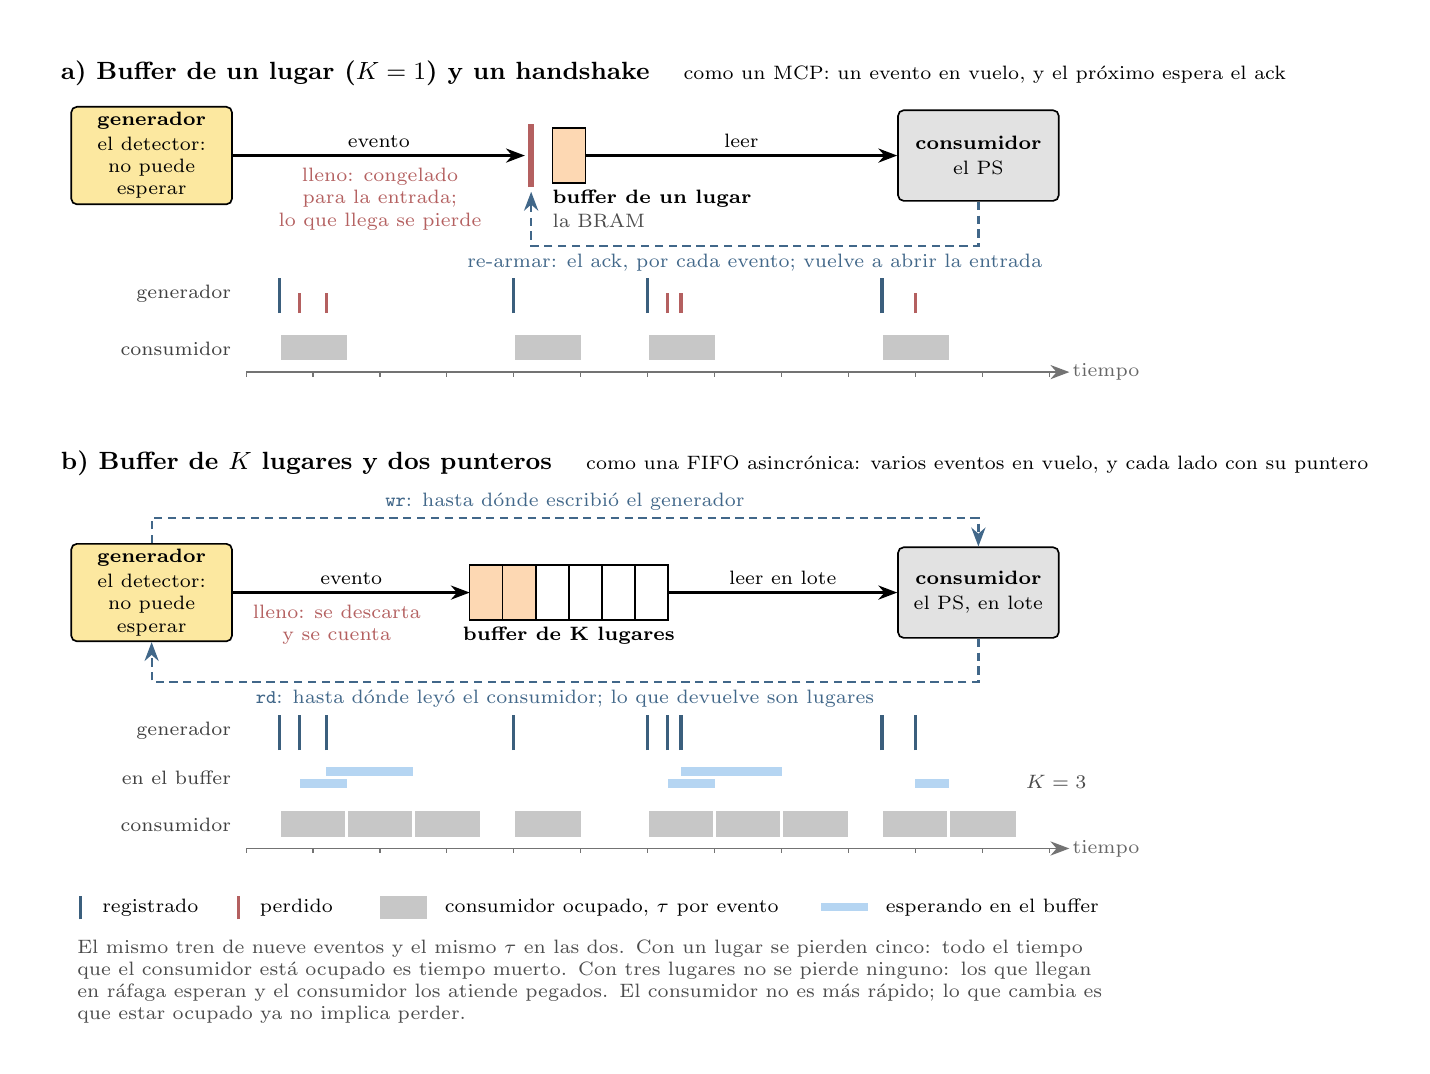
\begin{tikzpicture}[fondo]

% ===================================================== a) un lugar, handshake
\node[titulo] at (-0.4,0.75) {\textbf{a) Buffer de un lugar ($K = 1$) y un handshake}
  \quad {\scriptsize como un MCP: un evento en vuelo, y el próximo espera el ack}};

\node[trig, text width=1.9cm] (g1) at (0.9,-0.6) {\etq{generador}{el detector:\\ no puede esperar}};
\node[comp, text width=1.9cm] (c1) at (11.4,-0.6) {\etq{consumidor}{el PS}};
% el buffer: el mismo dibujo que en (b), con un solo lugar, ocupado
\draw[fill=naranja!80, line width=0.5pt] (5.99,-0.95) rectangle ++(0.42,0.7);
\node[font=\scriptsize\bfseries, anchor=north west, inner sep=1pt] at (5.95,-1.0) {buffer de un lugar};
\node[font=\scriptsize, black!70, anchor=north west, inner sep=1pt] at (5.95,-1.3) {la BRAM};
% lleno = congelado para la entrada: la compuerta se cierra hasta el re-armado
\draw[rojo!75!black, line width=2pt] (5.72,-1.0) -- (5.72,-0.2);
\draw[flujo] (g1) -- node[rotb, above=1pt] {evento} (5.64,-0.6);
\draw[flujo] (6.41,-0.6) -- node[rotb, above=1pt] {leer} (c1);
\node[pierde, anchor=north, align=center] at (3.8,-0.72) {lleno: congelado\\ para la entrada;\\ lo que llega se pierde};
\draw[ack] (c1.south) |- node[rotb, below=1pt, pos=0.75] {re-armar: el ack, por cada evento; vuelve a abrir la entrada} (5.72,-1.75) -- (5.72,-1.06);

% el tren, con un lugar
\carril{-2.35}{generador}
\carril{-3.05}{consumidor}
\foreach \t in {0.5, 4.0, 6.0, 9.5} {\arribo{\t}{-2.6}}
\foreach \t in {0.8, 1.2, 6.3, 6.5, 10.0} {\perdido{\t}{-2.6}}
\servicio{0.5}{1.5}{-3.2} \servicio{4.0}{5.0}{-3.2}
\servicio{6.0}{7.0}{-3.2} \servicio{9.5}{10.5}{-3.2}
\eje{-3.35}

% ===================================================== b) un buffer de K lugares
\begin{scope}[shift={(0,-5.55)}]
\node[titulo] at (-0.4,1.35) {\textbf{b) Buffer de $K$ lugares y dos punteros}
  \quad {\scriptsize como una FIFO asincrónica: varios eventos en vuelo, y cada lado con su puntero}};

\node[trig, text width=1.9cm] (g2) at (0.9,-0.6) {\etq{generador}{el detector:\\ no puede esperar}};
\node[comp, text width=1.9cm] (c2) at (11.4,-0.6) {\etq{consumidor}{el PS, en lote}};
% el buffer: seis lugares, dos ocupados
\foreach \i in {0,...,5} {
  \pgfmathsetmacro\xa{4.94+\i*0.42}
  \ifnum\i<2 \def\colb{naranja!80}\else\def\colb{white}\fi
  \draw[fill=\colb, line width=0.5pt] (\xa,-0.95) rectangle ++(0.42,0.7);
}
\coordinate (bi) at (4.94,-0.6);
\coordinate (bo) at (7.46,-0.6);
\node[font=\scriptsize\bfseries, anchor=north, inner sep=1pt] at (6.2,-1.0) {buffer de K lugares};
\draw[flujo] (g2) -- node[rotb, above=1pt] {evento} (bi);
\draw[flujo] (bo) -- node[rotb, above=1pt] {leer en lote} (c2);
\node[pierde, anchor=north, align=center] at (3.25,-0.72) {lleno: se descarta\\ y se cuenta};
% los punteros: cada lado es dueño del suyo y ve el del otro con atraso
\draw[puntero] (g2.north) -- ++(0,0.32) -| node[rotb, above=1pt, pos=0.25]
  {\texttt{wr}: hasta dónde escribió el generador} (c2.north);
\draw[puntero] (c2.south) -- ++(0,-0.55) -| node[rotb, below=1pt, pos=0.25]
  {\texttt{rd}: hasta dónde leyó el consumidor; lo que devuelve son lugares} (g2.south);

% el mismo tren, con K = 3
\carril{-2.35}{generador}
\carril{-2.95}{en el buffer}
\carril{-3.55}{consumidor}
\foreach \t in {0.5, 0.8, 1.2, 4.0, 6.0, 6.3, 6.5, 9.5, 10.0} {\arribo{\t}{-2.6}}
\espera{0.8}{1.5}{-3.08} \espera{1.2}{2.5}{-2.93}
\espera{6.3}{7.0}{-3.08} \espera{6.5}{8.0}{-2.93}
\espera{10.0}{10.5}{-3.08}
\servicio{0.5}{1.5}{-3.7} \servicio{1.5}{2.5}{-3.7} \servicio{2.5}{3.5}{-3.7}
\servicio{4.0}{5.0}{-3.7}
\servicio{6.0}{7.0}{-3.7} \servicio{7.0}{8.0}{-3.7} \servicio{8.0}{9.0}{-3.7}
\servicio{9.5}{10.5}{-3.7} \servicio{10.5}{11.5}{-3.7}
\eje{-3.85}
\node[font=\scriptsize, black!70, anchor=west, inner sep=1pt] at (\tx{11.6},-3.0) {$K = 3$};
\end{scope}

% =================================================================== leyenda
\begin{scope}[shift={(0,-10.3)}]
\draw[azul!55!black, line width=1.2pt] (0,0) -- ++(0,0.3);
\node[font=\scriptsize, anchor=west] at (0.15,0.15) {registrado};
\draw[rojo!75!black, line width=1.2pt] (2.0,0) -- ++(0,0.3);
\node[font=\scriptsize, anchor=west] at (2.15,0.15) {perdido};
\fill[black!22] (3.8,0) rectangle ++(0.6,0.3);
\node[font=\scriptsize, anchor=west] at (4.5,0.15) {consumidor ocupado, $\tau$ por evento};
\fill[azul!50] (9.4,0.1) rectangle ++(0.6,0.11);
\node[font=\scriptsize, anchor=west] at (10.1,0.15) {esperando en el buffer};
\node[font=\scriptsize, black!70, anchor=north west, text width=13.4cm, align=left, inner sep=0pt] at (-0.05,-0.25)
  {El mismo tren de nueve eventos y el mismo $\tau$ en las dos. Con un lugar se pierden
   cinco: todo el tiempo que el consumidor está ocupado es tiempo muerto. Con tres lugares
   no se pierde ninguno: los que llegan en ráfaga esperan y el consumidor los atiende
   pegados. El consumidor no es más rápido; lo que cambia es que estar ocupado ya no
   implica perder.};
\end{scope}

\end{tikzpicture}
\end{document}
